\chapter{Design}

\section{Indledning}
Formålet med design afsnittet er at beskrive hardwaren og softwaren for EKG-systemet. Det beskrives vha.  diagrammer og skitser som tydeligør, hvordan de forskellige klassers funktionalitet er, og hvordan klasserne snakker sammen.
  
\section{Hardware arkitektur}
I dette projekt er hardwaren blevet udleveret, derfor vil hardware arkitekturen ikke blive beskrevet ned i mindste detalje, men derimod kun hardwarens overordnede funktion. Hardwaren for systemet består af en National Instruments DAQ og en signalgenerator fra Analog Discovery. Disse er begge forbundet til en computer via USB-porte.
\\ 
I dette projekt bliver EKG-signalet ikke målt fysisk via en patient, men simuleret via et signal, som er hentet ned fra websiden PhysioNet \footnote{http://www.physionet.org}. 

\begin{figure}[H]
	\centering
	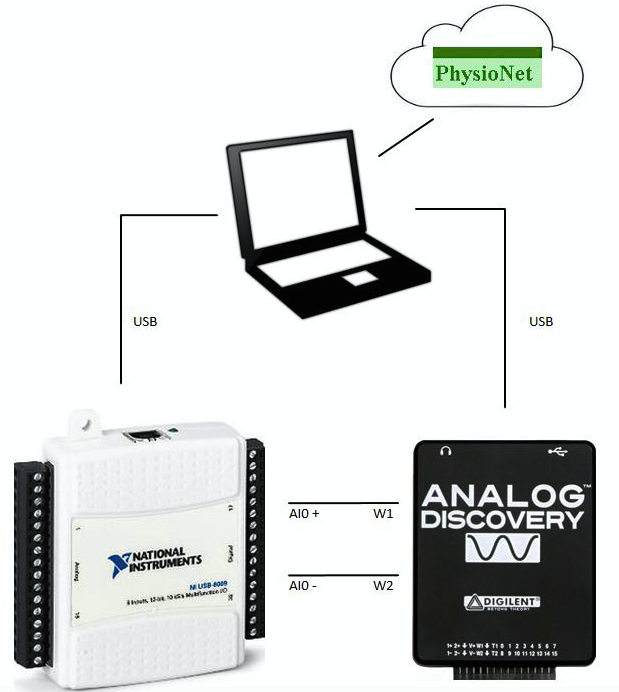
\includegraphics[width=0.6\textwidth]{Figurer/Snip20150427_1}
	\caption{Grafisk illustration af hardware opsætning}
\end{figure}

Som det ses på den overstående figur, er denne opstilling meget simpel. Figur 2.1 viser, hvordan de forskellige komponenter relaterer til hinanden. Display hardwaren vil i dette projekt være en computer, hvilket er et krav fra softwarens side, således at der kan vises et EKG-signal i form af en graf.
\\
\\  
Som beskrevet ovenfor er det Analog Discovery, som sammen med EKG-signalets informationer fra PhysioNet, skaber vores fiktive patient. Før EKG-signalet vises på computerens skærm, skal det igennem de forskellige komponenter i opstillingen. Analog Discovery modtager EKG-signalets  information som en CSV-fil, denne fil omdanner Analog Discovery til et analogt signal, som herefter sendes videre til DAQ’en. I DAQ’en digitaliseres det analoge signal, og tilpasses, så det efterfølgende kan udskrives på computer skærmen, i form af en EKG graf. 

\subsection{Græseflader}
Grænseflader af forbindelserne imellem de forskellige dele af hardwaren. 

\begin{table}[H] 
	\begin{tabularx}{\textwidth}{l l X}
    \toprule
     \textbf{Forbindelse}   & \textbf{Signaltype} & \textbf{Funktionalitet}    \\ \midrule
     DAQ - Computer         & Digital & DAQ'en konverterer det analoge signal til digitalt og videresender det til 							  computeren. Informationen sendes begge veje. \\ 
     					      \addlinespace[2mm]                                                                                                                                                                            
     Computer - Analog Discovery			& Digital & Computeren simulerer et EKG-signal og sender det til Analog Discovery.\\ 
     				    	  \addlinespace[2mm]   				                                                                                                                                                                           
     Analog Discovery - DAQ			   	& Analog & Analog Discovery	 konverterer signalet fra digitalt til analogt og videresender det til 							      DAQ'en.\\  				      
    \bottomrule                                                                                                                   
    \end{tabularx}
    \caption {Beskrivelse af grænseflader.}
    \label{tab:graenseflader}
\end{table}



\section{Software arkitektur}
I dette projekt arbejdes der med objektorienteret programmering i programmeringssproget C\#. Projektet er opbygget i henhold til trelagsmodellen, som er beskrevet i Rapporten under afsnittet Baggrund. Præsentationslaget består af 4 GUI’er, logiklaget af en enkelt klasse, og datalaget består af 3 klasser, hvoraf den ene er en blackbox.

\subsection{GUI}
I dette afsnit vil GUI’erne beskrives nærmere. Grafiklaget består i alt af 4 GUI’er eller vinduer - Login-vindue, CPR-vindue, EKG-vindue og Gem\_måling-vindue.

\begin{figure}[H]
	\centering
	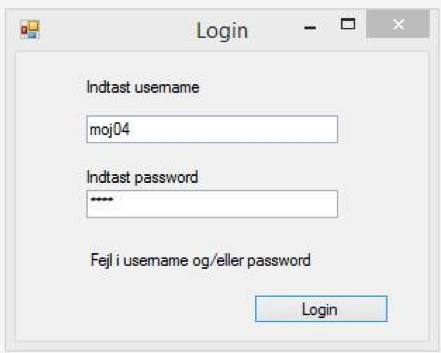
\includegraphics[width=0.8\textwidth]{Figurer/Snip20150430_38}
	\caption{Login-vindue}
\end{figure}

Når programmet startes op, vil et Login-vindue fremkomme på skærmen. Her skal brugeren logge ind for at få adgang til programmet, ved at indtaste sit personlige username og password. Bliver enten username eller password ikke godkendt, returneres en fejlmeddelelse, i form af en linje tekst nedenfor login-felterne. Bliver login godkendt åbnes CPR-vinduet.

\begin{figure}[H]
	\centering
	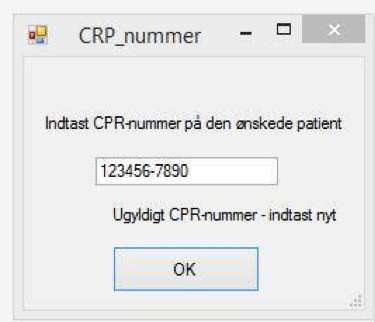
\includegraphics[width=0.6\textwidth]{Figurer/Snip20150430_39}
	\caption{CPR-vindue}
\end{figure} 

Her bliver brugeren bedt om at indskrive CPR-nummeret på den fiktive patient. CPR-nummeret bruges til at identificere personen i forbindelse med fremtidige målinger, samt til gemme målingerne i hvad der svarer til den fiktive persons journal. Hvis CPR-nummeret ikke bliver godkendt, vil brugerne blive gjort opmærksom på dette via en fejlmelding. 
\\
\\
Når CPR-nummeret bliver godkendt, åbner det primære vindue, EKG-vinduet. 

\begin{figure}[H]
	\centering
	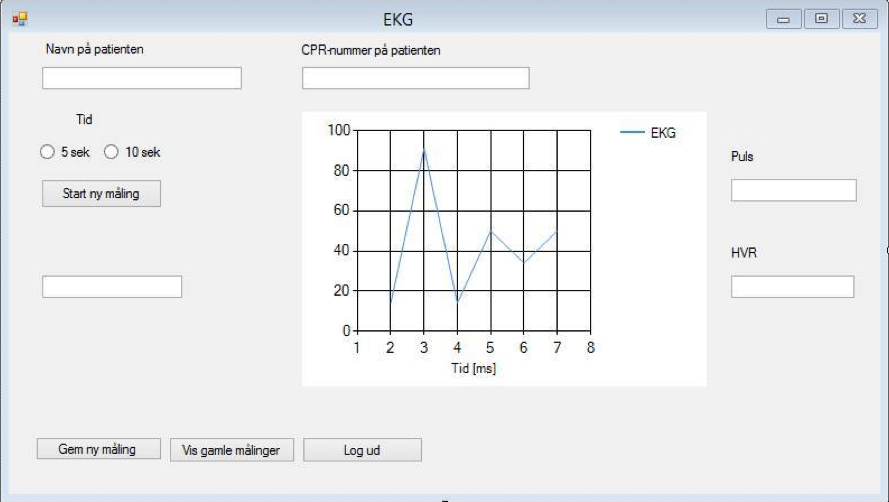
\includegraphics[width=1\textwidth]{Figurer/Snip20150430_40}
	\caption{EKG-vindue}
\end{figure}

EKG-vinduet er der, hvor man kan starte og se målinger. Vinduet er udstyret med knapper, som angiver hvor lang tid brugeren ønsker en måling skal køre over. Til højre i vinduet vises grafen over EKG-signalet, kort efter der er trykket ”Start ny måling”. Yderligere til højre kan der, i de to tekstbokse, ses puls og HVR for den pågældende graf. I det tomme tekstfelt, til venstre under knappen "Start ny måling", vil diagnosen for EKG-signalet udskrives. Nederst i vinduet er der knapper til at gemme målingerne, samt at logge ud fra programmet. Hvis man logger ud, kommer man tilbage til Login-vinduet, og EKG-vinduet er ikke længere synligt. 
\\
\\
Det sidste vindue der er valgbart, frembringes når der trykkes på ”Gem ny måling”. Herefter vises pop-up vindue, som bekræfter, at den pågældende EKG-målingen er gemt. 

\begin{figure}[H]
	\centering
	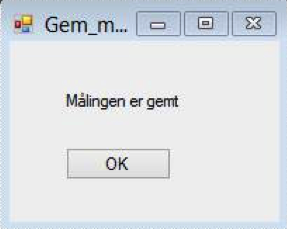
\includegraphics[width=0.5\textwidth]{Figurer/Snip20150430_41}
	\caption{Gem\_måling-vindue}
\end{figure}

\subsection{UML klassediagram}

\begin{figure}[H]
	\centering
	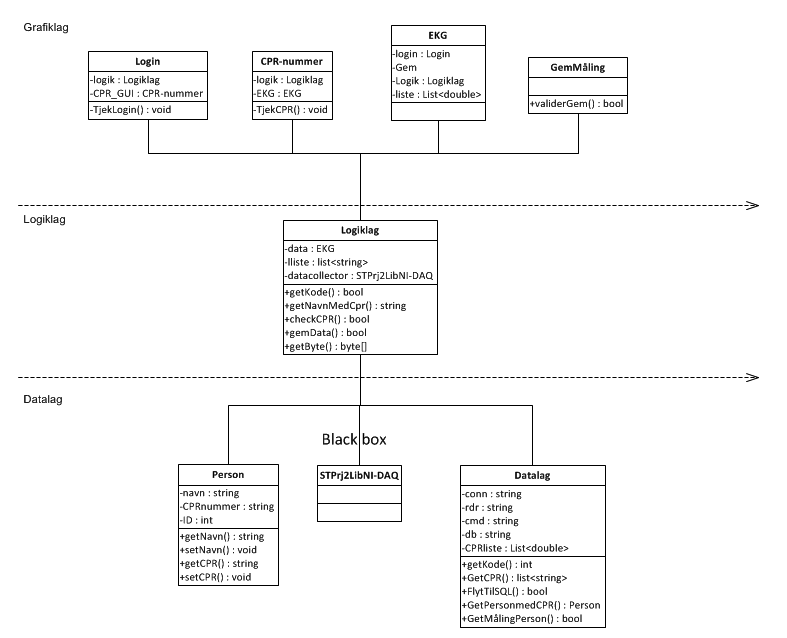
\includegraphics[width=1\textwidth]{Figurer/Snip20150430_42}
	\caption{UML-klassediagram over softwaren}
\end{figure}

Det ovenstående UML diagram over projektets software, giver en bedre og lettere forståelse for selve koden. Her er det meget tydeligt, at koden er opbygget efter trelagsmodellen. Præsentationslaget er bygget op af de førnævnte GUI’er, som bliver interfacen for selve bruger-interaktionen. I dette lag sker der som udgangspunkt intet behandlingsarbejde. Opsætningen og funktionerne af grafiklaget er yderligere beskrevet under afsnittet ’GUI’.\\ \\
Logiklaget består af en enkelt klasse, der fungerer som programmets primære styring. Logiklaget er til for, at grafiklaget ikke har direkte adgang til datalaget. Det er altså i dette lag alt programmets data bliver behandlet.  Her bliver EKG’et f.eks. analyseret og login, samt CPR, bliver valideret i forhold til det data, der ligger i datalaget. \\ \\
Datalaget består af to klasser, og en blackbox. I dette lag bliver der primært sørget for forbindelsen til databasen. Klassen ”Datalag” er kernen i dette lag. Her bliver der sørget for at gemme og hente informationer fra databasen. Det er i dette lag, hvor data’en som logiklaget arbejder med, kommer fra. Klassen ”Person”, er til for at binde alle person-informationer sammen, sådan at vi i stedet for at kalde 4 attributter, kan nøjes med at kalde et enkelt objekt. 

\subsection{Appliktationsmodel}
Applikationsmodel vil i almindelig forstand indeholde en overordnet domænemodel, herefter klassediagram samt sekvensdiagram og tilsidst et opdateret klassediagram, hvor metoderne fra sekvensdiagram er inkluderet. 

Applikationsmodellen for dette projekt består af en overordnet domænemodel, herefter sekvensdiagram for de forskellige Use Cases med tilhørende opdateret klassediagram, som beskriver metodekald og kommunikation mellem klasserne. Klassediagrammerne er undladt, da de er irrevalt for dokumentationen for projektet. Applikationsmodellen er udarbejdet udfra Use Cases, hvilket medfører at metoderne er fiktive, altså ikke hentet direkte fra softwaren.  

\subsubsection{Domænemodel}
Domænemodellen er skabt på baggrund af de fem Use Cases. Gennem navneordanalyse af Use Casene er de konceptuelle klasser fundet. I modellen beskrives, hvordan de konceptuelle klasser interagerer med hinanden. Controlleren er ikke en konceptuelle klasse, men er den, der sørger for at systemet fungerer optimalt.
\\
Der er ingen multiplicity indsat i modellen, da der kun arbejdes med et scenarie af gangen. !!!!!!!!!!!!!!!!!!!!!!!!!!!!!!!! spørg Lars 

\begin{figure}[H]
	\centering
	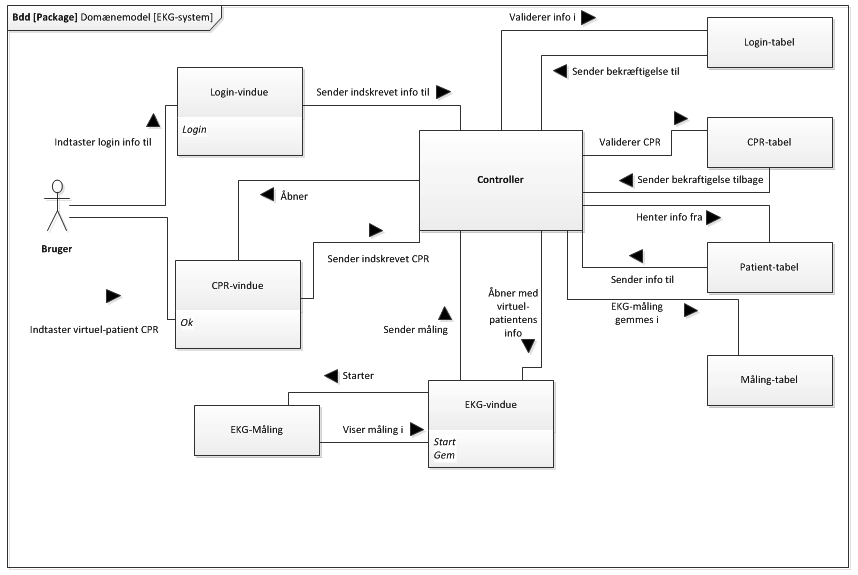
\includegraphics[width=1\textwidth]{Figurer/Snip20150429_37}
	\caption{Domænemodel af EKG-systemet}
\end{figure}

\subsubsection{Sekvensdiagram}
Sekvensdiagrammerne beskriver step-by-step via fiktive metoder forløbet i de forskellige Use Cases. Der er lavet et sekvensdiagram for hver Use Cases for at gøre systemet mere overskueligt. Et sekvensdiagram består af boundary-klasser og domain-klasser fra domænemodellen, samt en controller-klasse, som har navn efter den specifikke Use Case.  

\begin{figure}[H]
	\centering
	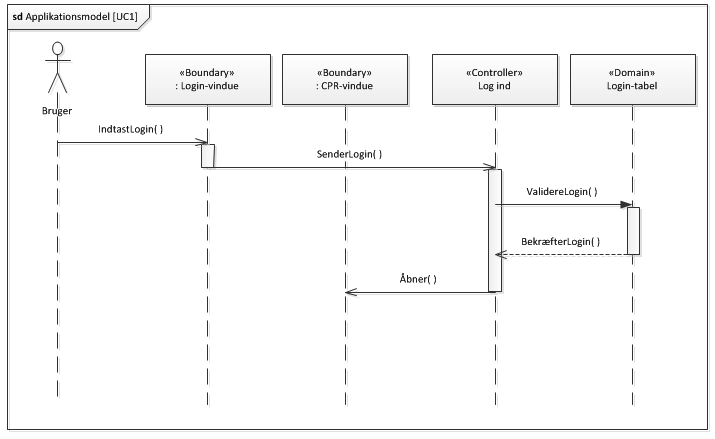
\includegraphics[width=0.9\textwidth]{Figurer/Snip20150429_34}
	\caption{Sekvensdiagram for UC1}
\end{figure}

\begin{figure}[H]
	\centering
	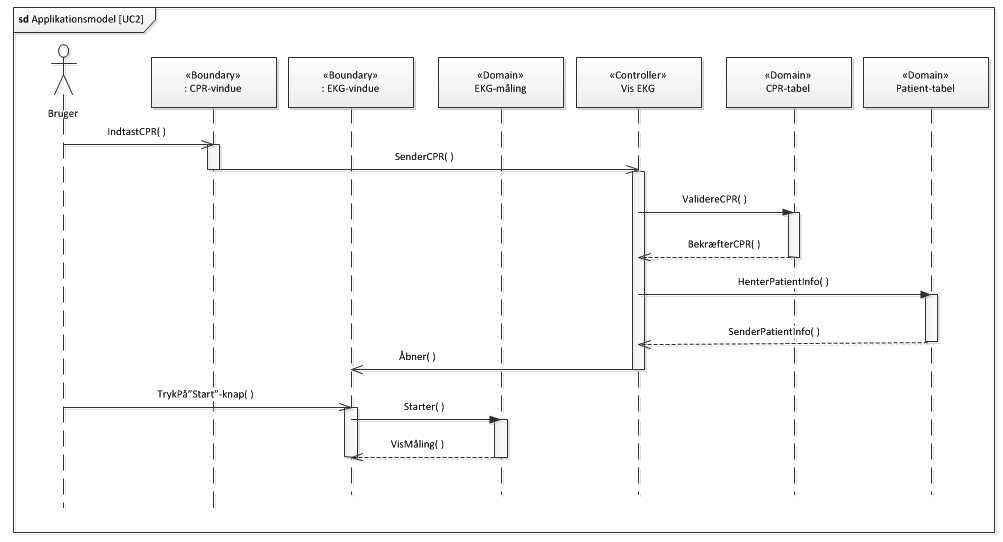
\includegraphics[width=1\textwidth]{Figurer/Snip20150429_33}
	\caption{Sekvensdiagram for UC2}
\end{figure}

\begin{figure}[H]
	\centering
	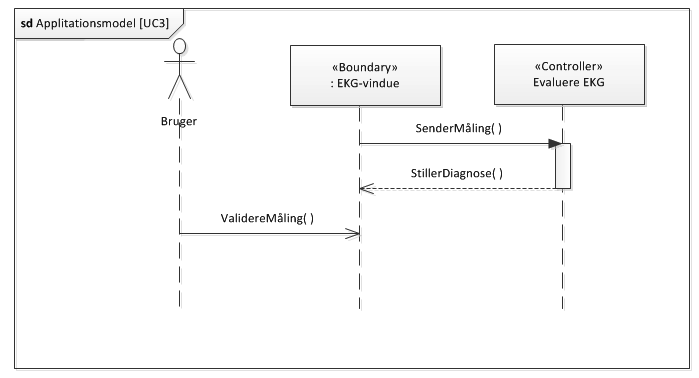
\includegraphics[width=1\textwidth]{Figurer/Snip20150429_31}
	\caption{Sekvensdiagram for UC3}
\end{figure}

\begin{figure}[H]
	\centering
	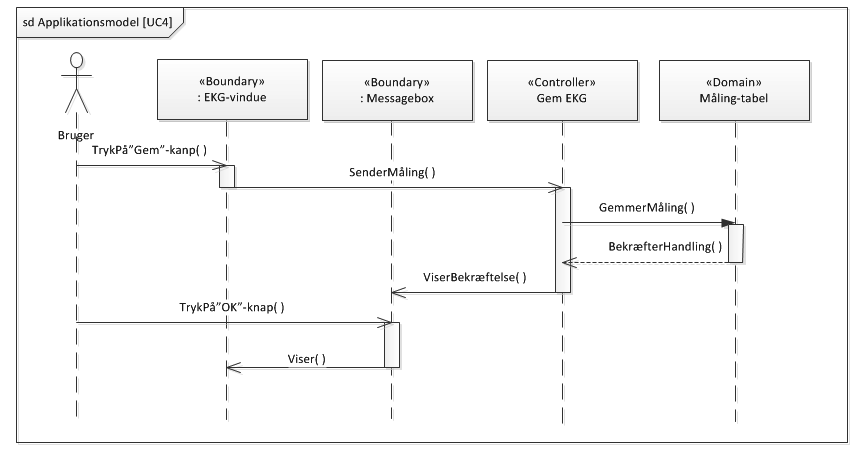
\includegraphics[width=1\textwidth]{Figurer/Snip20150429_28}
	\caption{Sekvensdiagram for UC4}
\end{figure}

\begin{figure}[H]
	\centering
	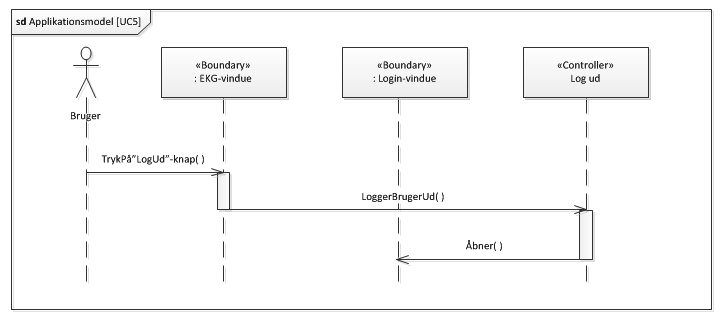
\includegraphics[width=1\textwidth]{Figurer/Snip20150429_30}
	\caption{Sekvensdiagram for UC5}
\end{figure}

\subsubsection{Opdateret Klassediagram}
De opdateret klassediagrammer indeholder metoderne fra de dertilhørende  sekvensdiagrammer - dette giver et overblik over, hvilke metoder de forskellige klasser består af.

\begin{figure}[H]
	\centering
	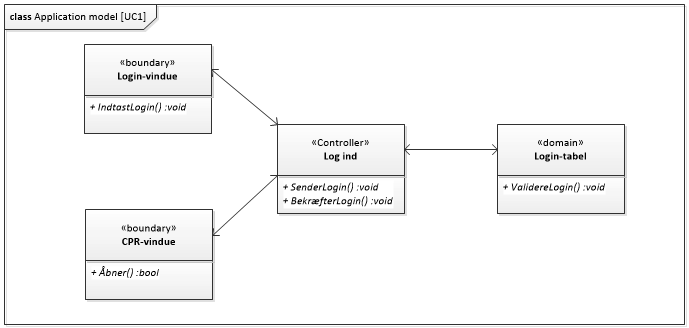
\includegraphics[width=1\textwidth]{Figurer/Snip20150429_20}
	\caption{Klassediagram for UC1}
\end{figure}  

\begin{figure}[H]
	\centering
	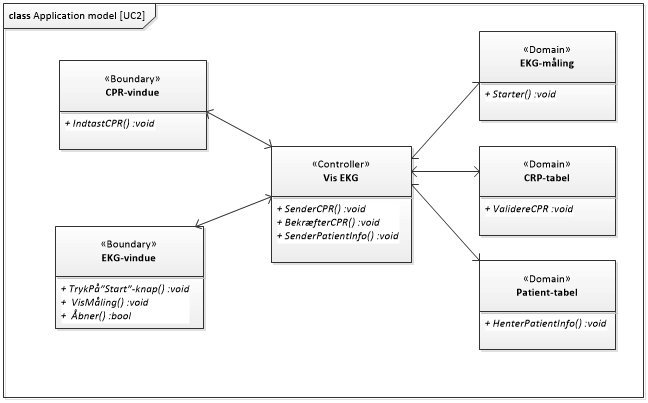
\includegraphics[width=1\textwidth]{Figurer/Snip20150429_22}
	\caption{Klassediagram for UC2}
\end{figure}

\begin{figure}[H]
	\centering
	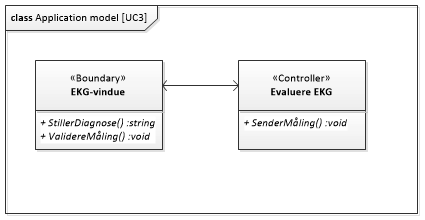
\includegraphics[width=1\textwidth]{Figurer/Snip20150429_23}
	\caption{Klassediagram for UC3}
\end{figure}

\begin{figure}[H]
	\centering
	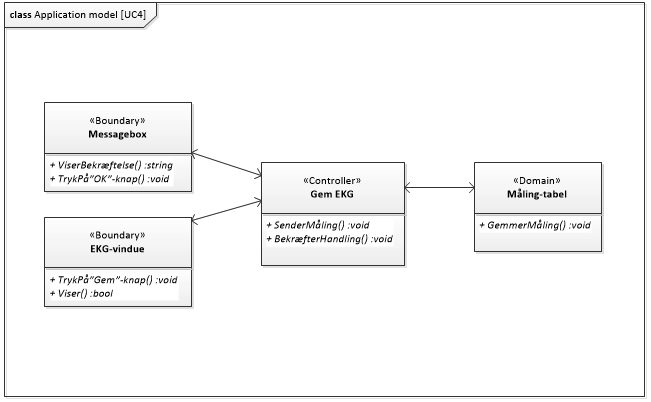
\includegraphics[width=1\textwidth]{Figurer/Snip20150429_26}
	\caption{Klassediagram for UC4}
\end{figure}

\begin{figure}[H]
	\centering
	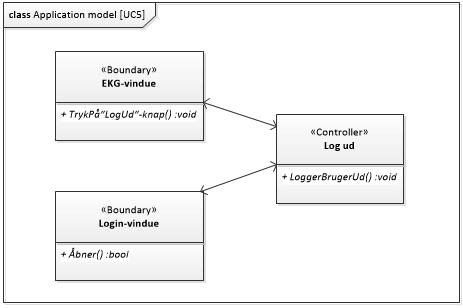
\includegraphics[width=1\textwidth]{Figurer/Snip20150429_25}
	\caption{Klassediagram for UC5}
\end{figure}





